\documentclass{article}

% 312 Font
\usepackage{charter}
% Circuit diagrams
\usepackage{circuitikz}
% Custom lists
\usepackage{enumitem}
% Page margins & pagestyles
\usepackage{fullpage}
% Font encoding
\usepackage[T1]{fontenc}
% Colored boxes around the 'solution' environment
\usepackage{mdframed}
% Used for making FSMs
\usepackage{tikz}
\usetikzlibrary{automata, arrows, calc, positioning}
% For color
\usepackage[dvipsnames]{xcolor}

% Defines a solution environment that creates a green box around text inside.
\mdfdefinestyle{SolutionFrame}{linecolor=green!60!black,linewidth=1pt}
\newenvironment{solution}{\begin{mdframed}[style=SolutionFrame]}{\end{mdframed}}

% Enumerate with (a),(b),(c),...
\newenvironment{enum}{\begin{enumerate}[label={(\alph*)}]}{\end{enumerate}}

% Put a dot after section titles
\renewcommand\thesection{\arabic{section}.}

% FSM config
\tikzset{
    ->,
    node distance=3cm,
    initial text=$ $,
}

% Images {img_size = 0.9, file_path}
\newcommand{\img}[2][0.9]{
    \begin{minipage}[t]{0.9\linewidth}
        \begin{center}
            \includegraphics[width=#1\linewidth]{#2}
        \end{center}
    \end{minipage}
}

% Hide the Date
\date{}
% Hide page numbers
\pagenumbering{gobble}

\begin{document}
    \begin{titlepage}
        \centering
        \null
        \vspace{5cm}
        {\Huge CSE 369 Lab 5\par}
        \vspace{0.5cm}
        {\Large Sequential Logic \par}
        \vfill
        {\hfill \Large Isaac Wu \par}
        {\hfill \large 2360957 \par}
        {\hfill \large \today \par}
    \end{titlepage}

\section{Finite State Machine}
    \begin{solution}
        \begin{center}
        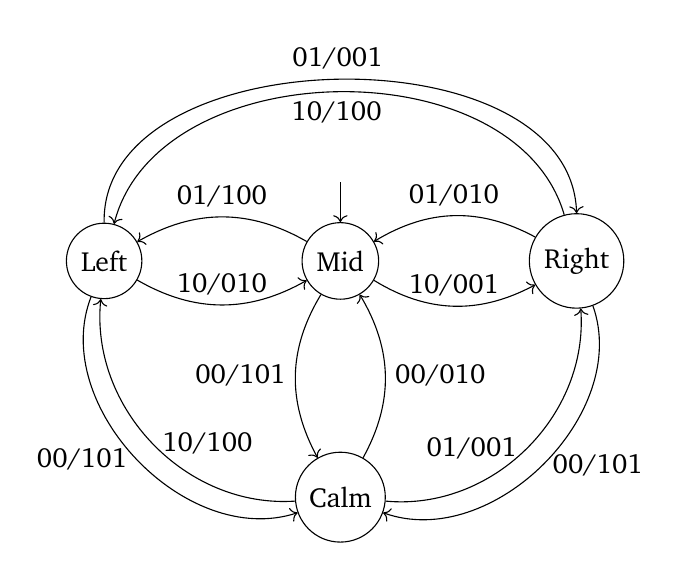
\begin{tikzpicture}
            \node[state, initial, initial where=above] (M){Mid};
            \node[state, left of=M] (L){Left};
            \node[state, right of=M] (R){Right};
            \node[state, below of=M] (C){Calm};

            \path
                % Init -> Calm
                (M)edge[bend right] node[left] {00/101}(C)
                (C)edge[bend right] node[right] {00/010}(M)
                
                % Init -> RL
                (M)edge[bend right] node[above] {01/100}(L)
                (L)edge[bend left=90] node[above] {01/001}(R)
                (R)edge[bend right] node[above] {01/010}(M)

                % Init -> LR
                (M)edge[bend right] node[above] {10/001}(R)
                (R)edge[bend right=75] node[below] {10/100}(L)
                (L)edge[bend right] node[above] {10/010}(M)

                % L -> Calm
                (L)edge[bend right=65] node[left] {00/101}(C)
                % R -> Calm
                (R)edge[bend left=65] node[right] {00/101}(C)

                % Calm -> L
                (C)edge[bend left=50] node[right] {10/100}(L)
                % Calm -> R
                (C)edge[bend right=50] node[left] {01/001}(R);
        \end{tikzpicture}
        \end{center}
    \end{solution}

\section{ModelSim Simulations}
    \begin{solution}
        This is the code for my runway light display.
        I defined my states in the enum and set their values to the LED pattern to display. \\
        I assign ledr to the present state instead of the next state so that a reset input is respected on the next clock cycle. I have the reset state be the middle state, since that LED pattern is common among all wind states. \\
        \img{runway.png}

        \newpage
        Here is the test bench used. I test each wind position and wait for some clock cycles to ensure correct LED behavior.
        \\
        \img{runway_tb.png}

        \newpage
        This is what the wave diagram looks like. The top wave is the clock used, it triggers the positive edge every 0.1ns. \\
        The second wave is the reset input, which is only true for the first clock cycle. \\
        The next 3 lines are the wind pattern inputs with switch inputs. \\
        The last 4 lines are the LED outputs. During each wind pattern, the LEDs cycle through each pre-defined display, shown on the bottom waves.
        \\
        \img[1.1]{waves.png}
    \end{solution}

\section{Resource Utilization by Entity}
    \img[1.1]{resource_utilization_by_entity.png}

\section{Misc.}
    How many hours (estimated) it took to complete this lab in total, including reading, planning, designing, coding, debugging, and testing.
    \begin{solution}
        It took around 3 hours to complete this lab.
    \end{solution}

\end{document}